In this chapter I will give an overview of how this audio codec will be designed, and explaining the various decisions I made along the way.

I have decided to call this new codec \emph{ANMF} (stands for Audio-NMF), using files with the extension \emph{.anmfx}, where \emph{x} represents the compression method.

There are currently three different ANMF formats that you can choose from, and their main difference is which audio representation is being compressed by NMF. They are as follows:

\begin{description}
	\item[ANMF-RAW] denoted by \emph{r}, compresses the signal in PCM form (time domain)
	\item[ANMF-MDCT] denoted by \emph{m}, compresses the signal transformed with MDCT (frequency domain)
	\item[ANMF-STFT] denoted by \emph{s}, compresses the signal transformed with STFT (frequency domain)
\end{description}

Our target output is a simple WAVE file, preserving samples in PCM form along with some metadata.

\section{WAVE file}
.. TODO ..

\section{Encoder}
The encoder is responsible for taking a raw audio file and encoding the data within, producing a compressed version of the original. Please refer to Figure \ref{fig:design_encoder} for a visual representation of the process.

\begin{figure}[ht]
	\label{fig:design_encoder}
	\caption[Encoder overview]{A high level overview of the ANMF audio encoder.}
	\centering
	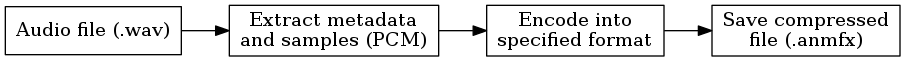
\includegraphics[width=\textwidth]{design_encoder.png}
\end{figure}

Next, each format's encoding process will be outlined (third step in the figure). If the audio file has multiple channels, this process is repeated on each channel separately.

\subsection{ANMF-RAW}
\begin{figure}[ht]
	\label{fig:encoding_nmf_raw}
	\caption[ANMF-RAW Encoder]{The encoding scheme for ANMF-RAW.}
	\centering
	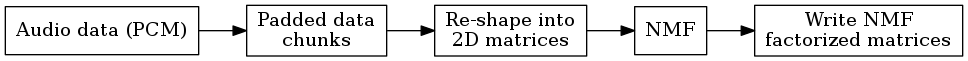
\includegraphics[width=\textwidth]{nmf_raw.png}
\end{figure}

.. TODO ..

\subsection{ANMF-MDCT}
\begin{figure}[ht]
	\label{fig:encoding_nmf_mdct}
	\caption[ANMF-MDCT Encoder]{The encoding scheme for ANMF-MDCT.}
	\centering
	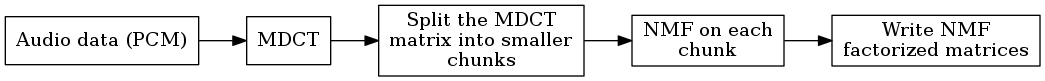
\includegraphics[width=\textwidth]{nmf_mdct.png}
\end{figure}

.. TODO ..

\subsection{ANMF-STFT}
\begin{figure}[ht]
	\label{fig:encoding_nmf_stft}
	\caption[ANMF-STFT Encoder]{The encoding scheme for ANMF-STFT.}
	\centering
	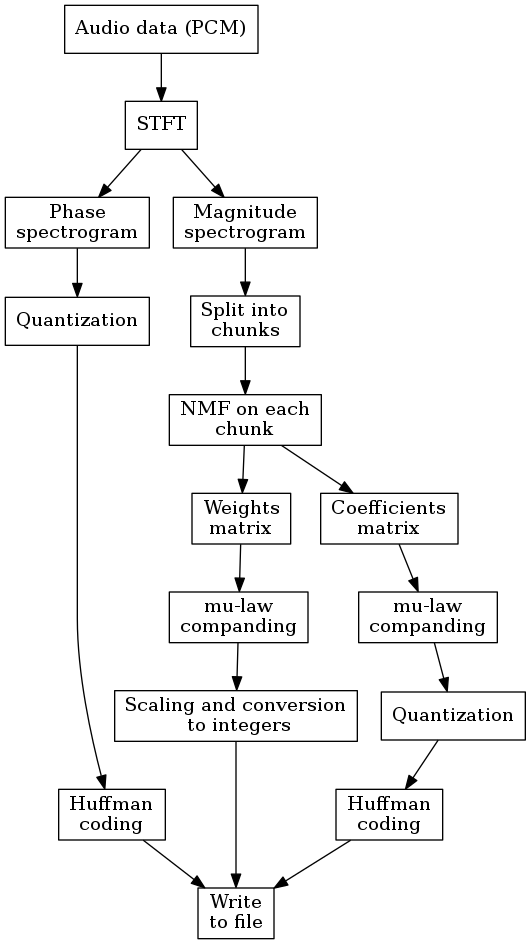
\includegraphics[width=0.6\textwidth]{nmf_stft.png}
\end{figure}

.. TODO ..

\section{Decoder}
Similar to the encoder, the decoder simply reverses the encoding process as seen in Figure \ref{fig:design_decoder}, and in each of the methods.

\begin{figure}[ht]
	\label{fig:design_decoder}
	\caption[Decoder overview]{A high level overview of the ANMF audio decoder.}
	\centering
	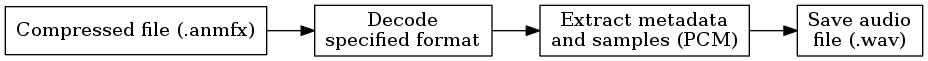
\includegraphics[width=\textwidth]{design_decoder.png}
\end{figure}

Next, each format's decoding process will be outlined.

\subsection{ANMF-RAW}
.. TODO ..

\subsection{ANMF-MDCT}
.. TODO ..

\subsection{ANMF-STFT}
.. TODO ..

mu-law quantization, non-uniform, formula in p128 wrong (missing sgn)\

- compressing MDCT

unusable, needs to be compressed consistently / losslessly

.. file structure ..

diagram for both time domain and frequency domain compression

